\documentclass[9pt,twocolumn,twoside,lineno]{gsajnl}
% Use the documentclass option 'lineno' to view line numbers

\usepackage{epstopdf}
\usepackage{subcaption}
\usepackage{verbatim}
\usepackage{booktabs}

\articletype{inv} % article type
% {inv} Brief Note
% {gs} Genomic Selection
% {goi} Genetics of Immunity
% {gos} Genetics of Sex
% {mp} Multiparental Populations

\newcommand{\beginsupplement}{%
\setcounter{table}{0}
\renewcommand{\thetable}{S\arabic{table}}%
\setcounter{figure}{0}
\renewcommand{\thefigure}{S\arabic{figure}}%
}

\runningtitle{GENETICS Journal Template on Overleaf} % For use in the footer
\runningauthor{Loay \textit{et al.}}

\title{Tuning the SMC: efficient simulation and the structure of ARGs}

\author[1,$\dagger$, $\ast$]{Hossameldin Loay}
\author[1, $\dagger$]{Gertjan Bisschop}
\author[2]{Derek Setter}
\author[3, 4]{Abdelmajid Omarjee}
\author[1,$\ddagger$]{Jerome Kelleher}
\author[2,$\ddagger$]{Konrad Lohse}

\affil[1]{
Big Data Institute, Li Ka Shing Centre for Health Information and Discovery, University of Oxford, Oxford, OX3 7LF, United Kingdom}
\affil[2]{Institute of Ecology and Evolution, University of Edinburgh, Edinburgh, UK}
\affil[3]{Institut de Syst´ematique, Evolution, Biodiversit´e UMR 7205 – Museum National d’Histoire Naturelle – France}
\affil[4]{Center for Interdisciplinary Research in Biology (UMR 7241) – Coll`ege de France, Paris Sciences et Lettres University, Paris – France}
\affil[$\dagger$]{Joint first author}
\affil[$\ddagger$]{Joint senior author}

% Use the \equalcontrib command to mark authors with equal
% contributions, using the relevant superscript numbers
%\equalcontrib{1}
%\equalcontrib{2}

\correspondingauthoraffiliation[$\ast$]{Corresponding author: hossam.ali@well.ox.ac.uk.}

\begin{abstract}
Sequentially Markovian Coalescent (SMC) models are a central element of
contemporary population genetics, underlying many inferential methods. While
the SMC has been shown to closely approximate the canonical Coalescent with
Recombination (CwR) in terms of low-dimensional, two-locus summaries, its
effects on the deeper structural properties of Ancestral Recombination Graphs
(ARGs) are less well understood. Here, we define a general SMC approximation,
SMC($k$), in which a single parameter $k$ controls the physical scale over
which common-ancestor events between non-overlapping ancestral segments are
permitted. The model encompasses the standard SMC and SMC$^\prime$ as special
cases and converges to the CwR as $k$ increases, providing a tunable trade-off
between computational efficiency and fidelity to the full recombination
process. Using recently developed summaries of ARG structure, we show that SMC
approximations systematically truncate the persistence of ancestral haplotypes
across the genome, despite preserving marginal coalescent properties, and that
increasing $k$ progressively recovers this long-range ancestral structure. We
implement the SMC($k$) in \texttt{msprime} and show that, for small samples, it
makes whole-chromosome simulation in species with large population-scaled
recombination rates, such as \emph{Drosophila melanogaster}, several orders of
magnitude faster than the CwR. Finally, we use SMC simulations for
chromosome-scale parametric bootstrapping of demographic inference and find
that SMC$^\prime$ captures uncertainty in SFS-based estimates remarkably well,
with only modest changes as $k$ increases despite substantial differences in
long-range ARG structure. Thus, the importance of SMC approximation error
depends strongly on which properties of ancestry are relevant to the downstream
analysis.
\end{abstract}

\keywords{Ancestral Recombination Graph; Tree sequence; Coalescent; SMC}


\begin{document}

\maketitle
\thispagestyle{firststyle}
\section{Introduction}

The coalescent with recombination (CwR) is the canonical mathematical framework
for modelling the ancestry of recombining sequences backwards in time
\citep{hudson_properties_1983,griffiths1997ancestral}. Although the CwR
captures the full stochastic process of recombination and common ancestry, its
complexity has long made both inference and simulation challenging.
\citet{mcvean_approximating_2005} introduced the Sequentially Markovian
Coalescent (SMC) as an approximation in which the sequence of local genealogies
forms a Markov process along the genome. Viewed backwards in time, this
approximation can be understood as restricting which ancestral lineages are
permitted to coalesce: under the standard SMC, common-ancestor events occur
only between lineages carrying overlapping ancestral material. The
SMC$^\prime$ refinement additionally permits adjacent ancestral
segments to merge \citep{marjoram_fast_2006}. The SMC and SMC$^\prime$
have since become standard models in population genetics and underpin a wide
range of inferential methods \citep{peede_not_2026}.

SMC approximations preserve the marginal distribution of local
genealogies, but
necessarily alter their dependence along the genome. How important these
differences are has classically been assessed using low-dimensional summaries
of linkage. Early work compared linkage disequilibrium in simulations
\citep[e.g.][]{mcvean_approximating_2005}, while later analytical results
showed that the SMC$^\prime$ provides an accurate approximation to the
joint distribution of pairwise coalescence times at two
loci~\citep{wilton_smc_2015}.
However, pairwise and two-locus summaries capture only part of the dependence
encoded by a complete Ancestral Recombination Graph (ARG), and it is less clear
how SMC approximations affect the persistence of ancestral haplotypes and other
long-range structural properties of ARGs.

Recent interest in ARG inference
\citep{brandt2024promise,lewanski2024era,nielsen2024inference,wong_general_2024}
has motivated new ways of describing and comparing the structure of inferred
and simulated ARGs. In particular, summaries based on the genomic spans
associated with ancestral nodes and on haplotype-based ARG similarity provide
information about ancestry that is not captured by local trees or pairwise
linkage statistics \citep{ignatieva2025length,fritze2026forest}. These
developments make it possible to revisit the accuracy of the SMC family at the
level of the ARG itself. This is increasingly relevant as population-genetic
analyses make greater use of long-range haplotype and genealogical
structure~\citep[e.g.][]{pope2026tracing},
for which agreement in marginal or two-locus distributions need not imply
agreement in the features of ancestry relevant to downstream inference.

An early application of SMC approximations was to provide faster simulations.
Early CwR simulators such as
\texttt{ms}~\citep{hudson2002generating} could not efficiently generate whole chromosomes
under human-like parameters, motivating approximate simulators based on the SMC
and related models \citep{marjoram_fast_2006,chen_fast_2009,staab_scrm_2015}. The introduction
of \texttt{msprime} \citep{kelleher_efficient_2016} largely removed this
computational advantage for human-like parameter regimes through an efficient
implementation of Hudson's CwR simulation algorithm. Over the past decade,
\texttt{msprime} has developed into a general platform for ancestry simulation
\citep{ragsdale2020lessons,baumdicker_efficient_2022,kelleher2020coalescent},
with support for models including the discrete-time Wright--Fisher process
\citep{nelson_accounting_2020}, explicit pedigrees
\citep{anderson-trocme_genes_2023}, and hybrid forward- and backwards-time
simulations \citep{kelleher2018efficient,haller2018tree,gopalan_bridging_2025}.
Its integration with \texttt{tskit} \citep{jeffery_population-scale_2026} also
provides efficient access to the resulting ARGs.
Nevertheless, the
computational cost of exact CwR simulation grows quadratically with
population-scaled recombination rate~\citep{baumdicker_efficient_2022},
and so whole-chromosome simulation can be
prohibitively expensive for species with
large population-scaled recombination rates,
such as \emph{Drosophila melanogaster}.


Here, we define a generalised SMC approximation, SMC($k$), in which the
parameter $k$ controls the maximum physical separation over which
common-ancestor events between non-overlapping ancestral segments are
permitted. The standard SMC and SMC$^\prime$ models arise as special cases, while
increasing $k$ progressively approaches the full CwR. Related approaches have
previously been used to trade approximation against simulation speed
\citep{chen_fast_2009,shlyakhter_cosi2_2014,staab_scrm_2015};
here, we use this generalisation
both as an efficient simulation model and as a controlled framework for
characterising what aspects of ARG structure are lost under SMC approximations.
We implement the SMC($k$) efficiently in \texttt{msprime} v1.4 and show that it
enables whole-chromosome simulation in high-recombination parameter regimes
that are prohibitively expensive under the CwR.
Using recently developed
summaries of ARG structure, we show that low-$k$ approximations truncate the
persistence of ancestral haplotypes along the genome, with CwR-like long-range
structure progressively recovered as $k$ increases. Finally, we illustrate how
these computational gains make previously impractical analyses possible by
using chromosome-scale SMC simulations to quantify uncertainty in demographic
inference through parametric bootstrapping in \emph{D.\ melanogaster}.
Despite substantial differences in long-range ARG structure, we find that
the SMC$^\prime$ captures uncertainty in SFS-based demographic estimates remarkably
well, illustrating that the practical importance of SMC approximation error
depends on the properties of ancestry relevant to the downstream analysis.


\section{Results}
\label{sec:materials:methods}

\begin{figure}[t] \centering
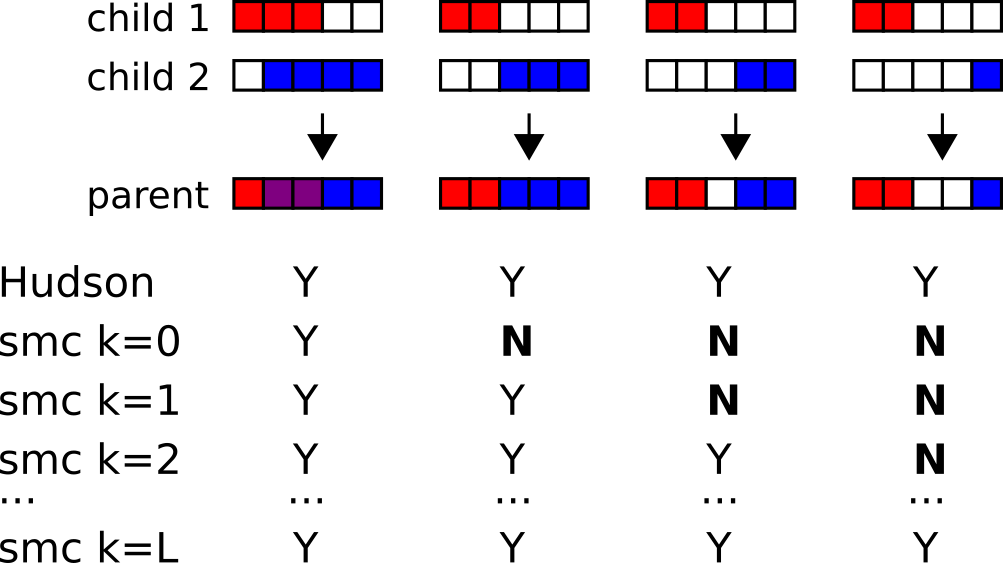
\includegraphics[width=0.8\linewidth]{figures/smck_illustration.png}
\caption{\textbf{The SMC(k) model restricts common ancestry events.} We indicate
which of the possible common ancestor events are permitted for various choices of
$k$. All scenarios are allowed under the CwR. For $k = 0$ (SMC), common ancestry (purple)
is permitted only when the lineages carry overlapping ancestral
material (red and blue). For $k=1$ (SMC'), common ancestry
may also occur if adjacent intervals are present.
For $k>1$, common ancestry events that result in trapped non-ancestral material are
permitted. The maximum span of any such interval is $k-1$, and when $k=L$, the
full sequence length, the model converges to the CwR.}
\label{fig:illustration1} \end{figure}

\begin{figure} \centering 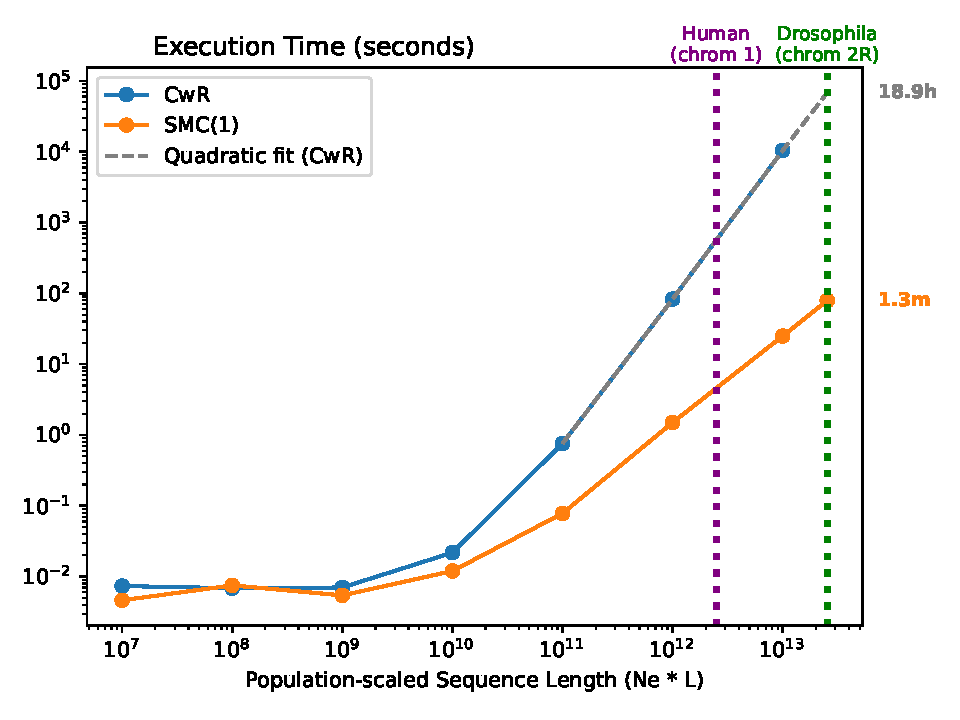
\includegraphics[width=\linewidth]{figures/speed.pdf}
\caption{\textbf{The SMC($k$) enables whole chromosome simulations in the
\textit{Drosophila} parameter regime}. Execution time for simulations under the
CwR and the SMC(1) model for a sample of $n=2$ diploid sequences and assuming
different population-scaled sequence length for chromosome 1 in humans ($10e4
\times 249Mbp$) and chromosome 2R \textit{D.\ melanogaster} $10e6 \times
25.4Mbp$.} \label{fig:speed} \end{figure}

\begin{figure}[t] \centering
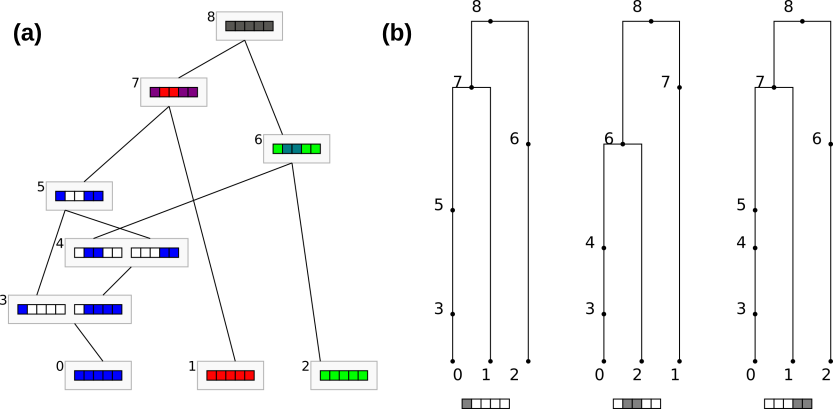
\includegraphics[width=\linewidth]{figures/arg_illustration.png}
\caption{\textbf{The ancestry of a sample of three haplotypes in ARG format
(left) and treesequence format (right).} In the ARG, we see that nodes 3 and 4
both have two parents, meaning they are recombinant nodes. These recombination
events result in three distinct correlated trees along the genome. Coalescence
in ancestral node 5 results in trapped non-ancestral material. It is (locally)
unary in the left and right trees but absent in the middle tree. Subsequent
coalescence in node 7 results in a node that is binary for the left and right
trees, but unary in the middle tree. This type of event is possible only under
the CwR or the SMC(k) with k $\geq$ 3.} \label{fig:illustration2} \end{figure}

\subsection{The SMC(k) model}

The SMC models the ancestry of a sample by assuming a Markovian process along
the genome, such that the local genealogy at any position depends only on the
genealogy immediately to its left \citep{mcvean_approximating_2005}. Backwards
in time, the standard SMC has an equivalent formulation in which common
ancestor events are restricted to pairs of lineages carrying overlapping
ancestral material
\citep{mcvean_approximating_2005,bisschop_likelihoods_2025}.
This restriction excludes common ancestor events that generate trapped,
non-ancestral material \citep{wiuf1999ancestry}, causing the SMC to
overestimate the number of independent ancestors contributing to a sample and
to underestimate long-range linkage disequilibrium
\citep{marjoram_fast_2006}. For example, under the CwR, two lineages created by
a recombination event may subsequently coalesce back together before further
events alter their ancestry.
The SMC$^\prime$ restores these
``diamonds''~\citep{rasmussen2014genome}
by additionally permitting common ancestor events between exactly adjacent,
but non-overlapping, ancestral segments \citep{marjoram_fast_2006}. This
backwards-time formulation suggests a natural family of intermediate
approximations in which common ancestor events are permitted over a
genomic scale.

We define the SMC($k$) by associating each ancestral lineage with the genomic
``hull''
of the ancestral material that it carries, spanning its leftmost to rightmost
ancestral segment. A common ancestor event between lineages $a$ and $b$ is
permitted only when the physical distance between their hulls is at most $k$
(Fig.~\ref{fig:illustration1}). Thus, $k$ determines the maximum genomic scale
over which separated ancestral material can be brought together by a common
ancestor event. Importantly, the SMC($k$) modifies only which common ancestor events
are permitted; recombination events occur at the same local rates as under the
CwR. On a genome with discrete coordinates and a sequence length of $L$
base pairs,
SMC(0) is equivalent to the standard SMC, and
SMC(1) to the SMC$^\prime$, while SMC($L$) recovers the full CwR.
Increasing $k$ therefore gives a nested sequence of
models in which progressively more of the common ancestor events possible
under the CwR are retained. Consequently, increasing $k$ permits progressively
longer spans of trapped non-ancestral material (Fig.~\ref{fig:illustration1}).
Related approaches to controlling the extent of the SMC approximation have
previously been implemented in \textit{MaCS} \citep{chen_fast_2009},
\textit{scrm} \citep{staab_scrm_2015}, and \textit{Cosi2}
\citep{shlyakhter_cosi2_2014}.

We implemented the SMC($k$) in \texttt{msprime} v1.4 by extending its existing
backwards-time CwR simulation algorithm~\citep{kelleher_efficient_2016}. In
addition to the linked list of ancestral segments maintained for each lineage,
the SMC($k$) implementation records the hull of each extant lineage.
Hull endpoints are maintained in ordered search structures, allowing the simulator
to identify eligible common-ancestor pairs without explicitly testing all
possible lineage pairs after each event. A separate cumulative index stores,
for each lineage, the number of eligible common-ancestor partners and allows
common-ancestor events to be sampled efficiently.
The sum of these counts determines the rate of common ancestor events, and when
such an event occurs a pair is sampled uniformly from the set of eligible
pairs. Recombination and common ancestor events can change the extent of the
ancestral material carried by a lineage, in which case its hull and the
corresponding pair counts are updated. Thus, relative to Hudson's CwR
algorithm, the principal additional cost of the SMC($k$) is maintaining the search
indexes that identify eligible common-ancestor pairs.

This additional bookkeeping leads to a different computational regime from the
standard CwR algorithm. For modest sample sizes and very large
population-scaled recombination rates, the SMC($k$) can provide substantial gains
over the CwR.
For example, simulating two diploid samples for the entirety of
\emph{Drosophila melanogaster} chromosome 2R under
SMC(1) is approximately three orders of magnitude faster than under the CwR
(Fig.~\ref{fig:speed}). This makes chromosome-scale simulations feasible in a
parameter regime in which exact CwR simulations are prohibitively expensive.
The advantage is not universal, however.
Over the range tested,
execution time for
SMC(1) scales approximately linearly with sample size, whereas the
corresponding CwR simulations scale approximately logarithmically
(Supplementary Figs.~\ref{fig:speed_per_sample_size}, \ref{fig:scaling_sample_size}).
The computational advantage of the SMC($k$) also diminishes as $k$ increases.
Consequently, the SMC($k$) is most useful for long sequences with large
population-scaled recombination rates and relatively modest sample sizes; for
large samples or sufficiently large $k$, the standard CwR implementation can
be more efficient.

\subsection{Long-range ARG structure under SMC approximations}

The SMC$^\prime$ is widely regarded as a highly accurate approximation to the
CwR, supported by the close agreement between the two models in the joint
distribution of pairwise coalescence times at two loci
\citep{wilton_smc_2015}. Expectations for standard two-locus summaries of
linkage disequilibrium can be expressed in terms of the covariance in pairwise
coalescence times \citep{mcVean2002genealogical}, but such summaries capture
only part of the dependence encoded by a complete ARG. In particular, close
agreement in two-locus quantities does not establish whether SMC approximations
preserve the long-range persistence of ancestry across the genome. To
characterise these differences directly, we therefore consider structural
properties of the nodes contained in ARGs generated under the SMC($k$) and the
CwR.

Each node in an ARG corresponds to a unique genetic ancestor of the sample, and
the genomic material associated with a node can be divided into three
categories (Fig.~\ref{fig:illustration2}). The binary span of a node is the
total genomic span over which an ancestor contributes to two child nodes.
Analogously, the unary span is the total genomic span over which an ancestor
has a single child node \citep{wong_general_2024}. Unary structure captures
the persistence of ancestral lineages across neighbouring local genealogies
and is increasingly recognised as an important component of overall ARG
structure
\citep{bisschop_likelihoods_2025,fritze2026forest}. Finally, trapped
non-ancestral material consists of genomic intervals lying between binary
and/or unary segments associated with the same node. A single common ancestor
node may therefore contribute to more than one span category. For example,
node 5 in Fig.~\ref{fig:illustration2} is binary over two genomic segments
separated by trapped non-ancestral material, whereas node 7 is binary over the
same two segments but unary across the intervening interval. Together, these
span measures describe how ancestral lineages persist across the genome in
ways that are not captured by the sequence of local trees alone.

We simulated ARGs under the SMC($k$) for a range of $k$ values and compared the
resulting node spans with those generated under the CwR. Across the scaled
recombination rates considered, low-$k$ approximations produce systematically
shorter unary spans than the CwR
(Fig.~\ref{fig:stacked_bar}). Binary spans show the same qualitative pattern
(Supplementary Fig.~\ref{fig:avg_l2_log}), and similar results are obtained for
larger samples. These differences indicate that ancestral lineages persist
across shorter genomic distances under the SMC($k$). As $k$ increases, both
unary and binary spans progressively approach those observed under the CwR,
while increasingly long intervals of trapped non-ancestral material become
possible. Thus, common ancestor events between separated genomic segments,
although contributing relatively little to pairwise coalescence-time
correlations, make an appreciable contribution to the long-range persistence
of ancestral material in a complete ARG.

We next compared the overall ancestral structure of ARGs using ``matched
span'', a similarity measure implemented in \textit{tscompare}
\citep{fritze2026forest}. We normalised matched-span similarity by the
baseline similarity expected between independently simulated CwR ARGs. The
fraction of CwR ancestral structure matched by SMC($k$) ARGs increases with
$k$, approaching the CwR baseline as progressively more common ancestor events
are permitted (Fig.~\ref{fig:ts_inverse_matched_span}). In contrast, the
reciprocal comparison shows little dependence on $k$: ancestral structure
present in SMC($k$) ARGs is generally also represented in CwR ARGs
(Supplementary Fig.~\ref{fig:ts_matched_span}). Together, these results are
consistent with the SMC($k$) generating a restricted subset of the ancestral
structures produced under the CwR, with low-$k$ approximations primarily
removing long-range ancestral relationships rather than introducing
qualitatively different structures.

\begin{figure}[t] \centering
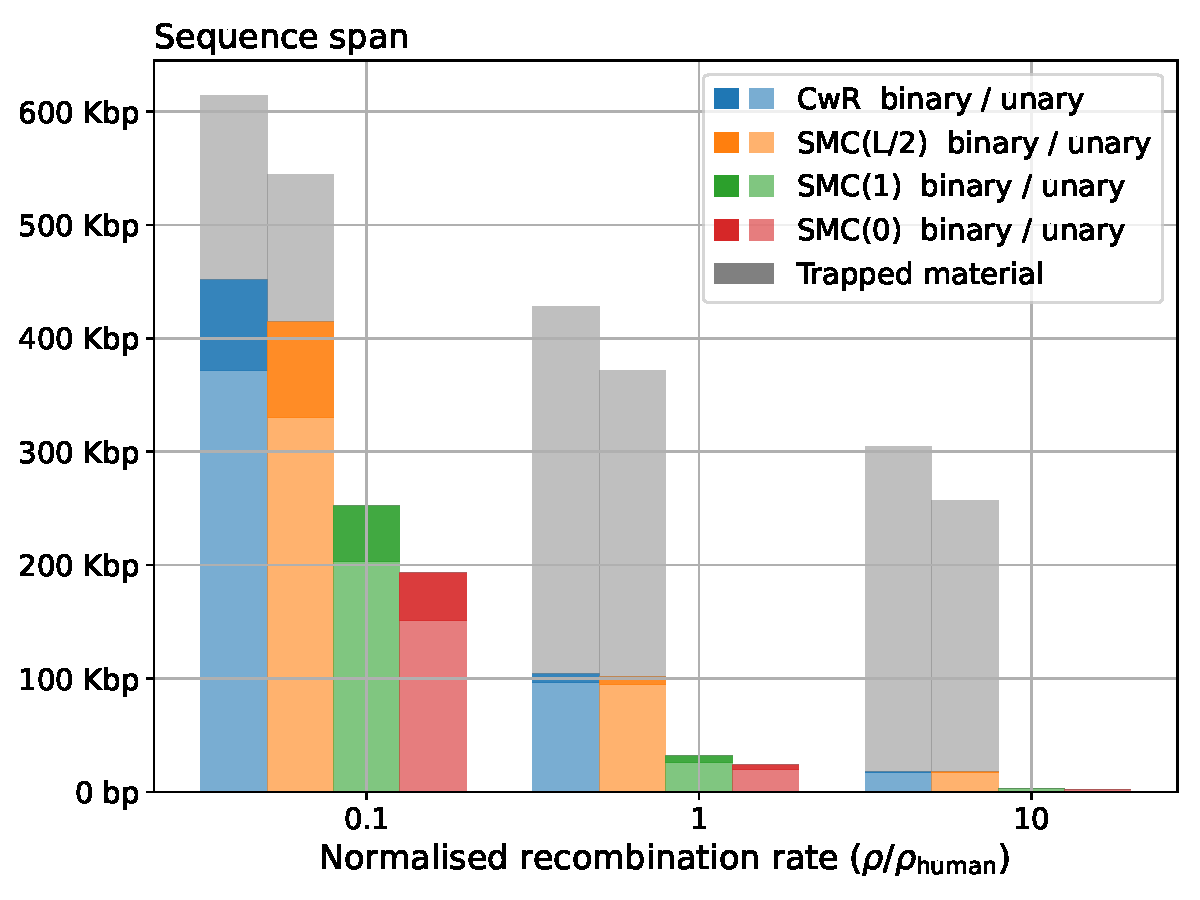
\includegraphics[width=\linewidth]{figures/average_hulls_2samples_segments_stacked_bar.pdf}
\caption{\textbf{The distribution of ancestral material differs between the
SMC' and CwR models}. Stacked bars show the average sequence span per node of
unary nodes (lighter colours), binary nodes (darker colours), and trapped
non-ancestral material (grey) across human-scaled recombination rates for
different models. ARGs that arise from the SMC' and standard SMC model do not
contain trapped non-ancestral material by definition. The simulated chromosome
is of 1 Mbp length. (CwR in blue, SMC(0) in red, SMC(1) in green, and SMC(L/2)
in orange).} \label{fig:stacked_bar} \end{figure}

\begin{figure} \centering
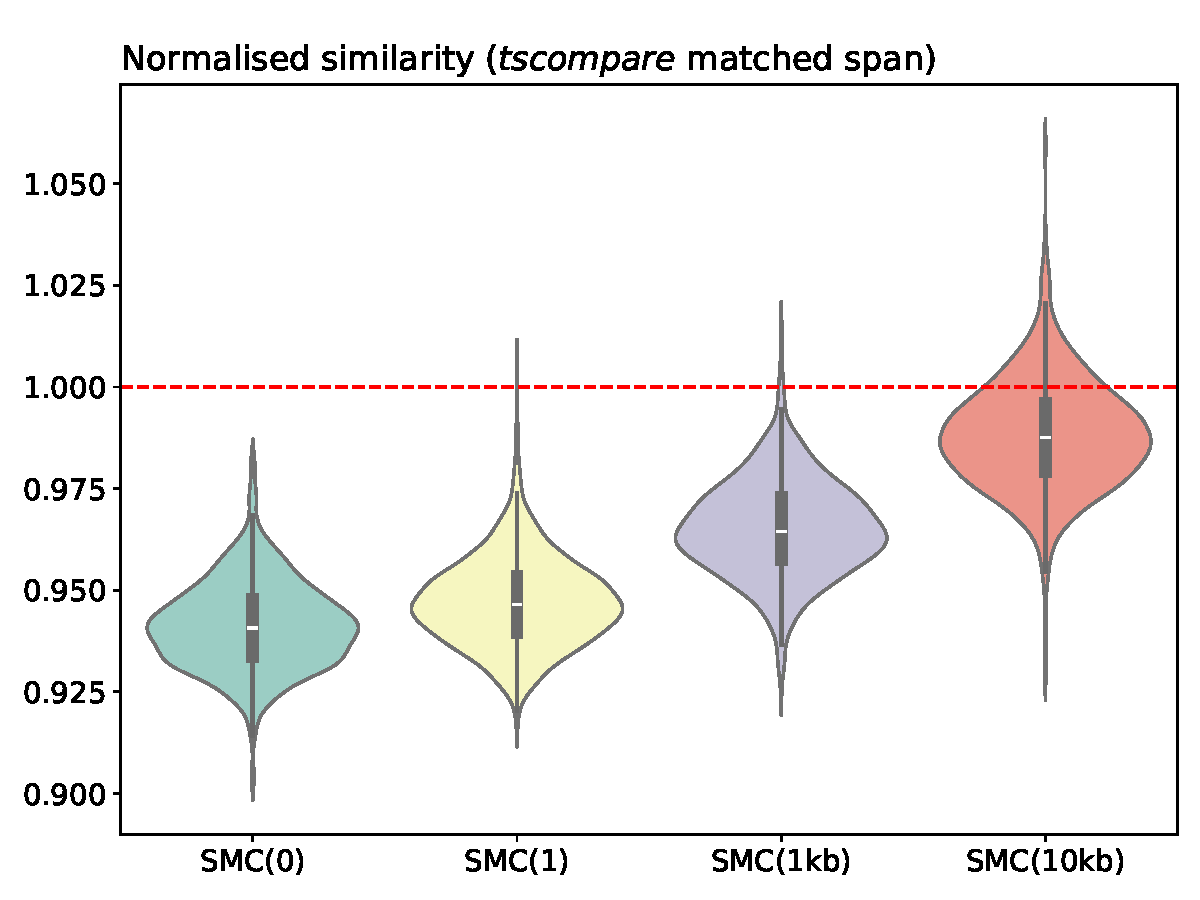
\includegraphics[width=\linewidth]{figures/tscompare_inverse_matched_span_length_comparison.pdf}
\caption{\textbf{The similarity between ARGs simulated under the CwR and the
SMC(k) depends on $k$.} The distribution of normalised similarity between ARGs
simulated under the CwR and SMC(k) for different values of $k$. Similarity is
measured in terms of the \texttt{matched span} length computed by
\textit{tscompare} normalised by the similarity expected between two random
ARGs simulated under the CwR.} \label{fig:ts_inverse_matched_span} \end{figure}

\subsection{Bootstrapping demographic inference}
% JK: On finishing this section I'm left wondering how the msprime simulations
% helped here. Can we add some quantitive detail here on the number of
% simulations performed, how long they took, and how long they might have
% taken under the CwR?

Drawing inferences about the demographic and selective history of populations
is a key goal in population genomics. Many inference tools focus on variation
at the level of SNPs which can be summarised via the site frequency spectrum
(SFS) or higher order summaries thereof \citep{gutenkunst_inferring_2009,
excoffier_fastsimcoal2_2021, liu_stairway_2020, omarjee_blockbuster_2026}.
While SFS based inference of point estimates in a composite likelihood
framework is efficient, it ignores LD between variants. Similarly, inference
methods based on variation within sequence blocks
\citep{laetsch_demographically_2023} or loci also tend to assume statistical
independence between them. In both cases, quantifying the uncertainty in
composite likelihood estimates has proven challenging, and solutions to this
problem generally rely on an arbitrary cut-off. That is, one assumes that SNPs
or sequence blocks separated by some minimal physical or map distance can be
treated as (approximately) statistically independent. The alternative is to
perform a data bootstrap with a scale of block-wise resampling that is
generally not informed by LD.

This use of distance thresholds -- albeit common practice in the field -- is
clearly \emph{ad hoc} and not justifiable given that under the CwR, LD is
non-zero even between pairs of loci on opposite ends of a chromosome. As a
consequence, it is generally unclear whether confidence intervals based on such
thresholds are conservative or overconfident. A meaningful estimation of
uncertainty of composite likelihood parameters must incorporate the statistical
non-independence of genomic variation due to LD, and the SMC(k) provides the
means to do this even for organisms with high recombination rates.

To demonstrate how simulations under the SMC(k) can be used to achieve this, we
perform parametric boostraps for the inference of a piecewise constant history
of $N_e$ change in the South African \textit{D.\ melanogaster} population (SP)
from WGS data ($n =38$ individuals \citep{pool2012}) first described by
\citet{chen_sub-saharan_2024}. This history was initially inferred from the
unfolded SFS of putatively neutral sites on chromosome 2R (which is free of
large inversions) using Stairway Plot 2 \citep{liu_stairway_2020}. To perform a
parametric bootstrap for the inferred demographic history, we simulated
replicated datasets under the inferred history using SMC(1). For each
replicate, we used \texttt{blockbuster} \citep{omarjee_blockbuster_2026}, an
analytic composite likelihood method analogous to but more efficient than
Stairway Plot 2, to infer a three epoch model of $N_e$ change from the SFS (see
Methods, code available in xxx).

We find that, as expected, the uncertainty in estimated $N_e$ was lowest for
the middle epoch (blue in Fig.\ \ref{fig:bootstrap} right). Since low values of
$k$ underestimate long range LD, one would expect an associated underestimation
of the uncertainty in point estimates of $N_e$. However, while our bootstrap
analysis (Supplementary Fig.\ ~\ref{fig:error_decay_analysis}) shows the
expected increase in uncertainty (measured in terms of mean squared error) with
$k$, we find that this effect is surprisingly small.

% TODO merge this in here. In particular, we're not referencing fig:variance.

% It is perhaps surprising that the expected uncertainty in estimates of
% population size change based on the SMC' are very similar to that of the full
% CwR. We conclude that parametric bootrapping based on the SMC' is sufficient
% for SFS based estimates of stepwise constant histories. Nevertheless,
% bootstrapping based on the SMC' model is slightly overconfident, i.e.\
% underestimates uncertainty in parameter estimates compared to the full CwR
% model (Supplementary Fig.~\ref{fig:variance}). We would argue that the accuracy
% of bootstrapping based on SMC(k) (and the choice of $k$) must depend both on
% the demographic history at hand and the data summary one considers. Long-range
% LD that is generated, for example, under demographic histories that include
% recent gene flow is unlikely to be captured well with low values of $k$.
% Indeed, bootstrapping for inference based on haplotype summaries or Hidden
% Markov Models (which themselves assume the SMC') likely requires more accurate
% modelling of long-range LD, and so higher $k$. Further work is required to
% determine how the accuracy of parametric bootstrap depends on model complexity
% and data summaries.


\begin{figure*}
\centering
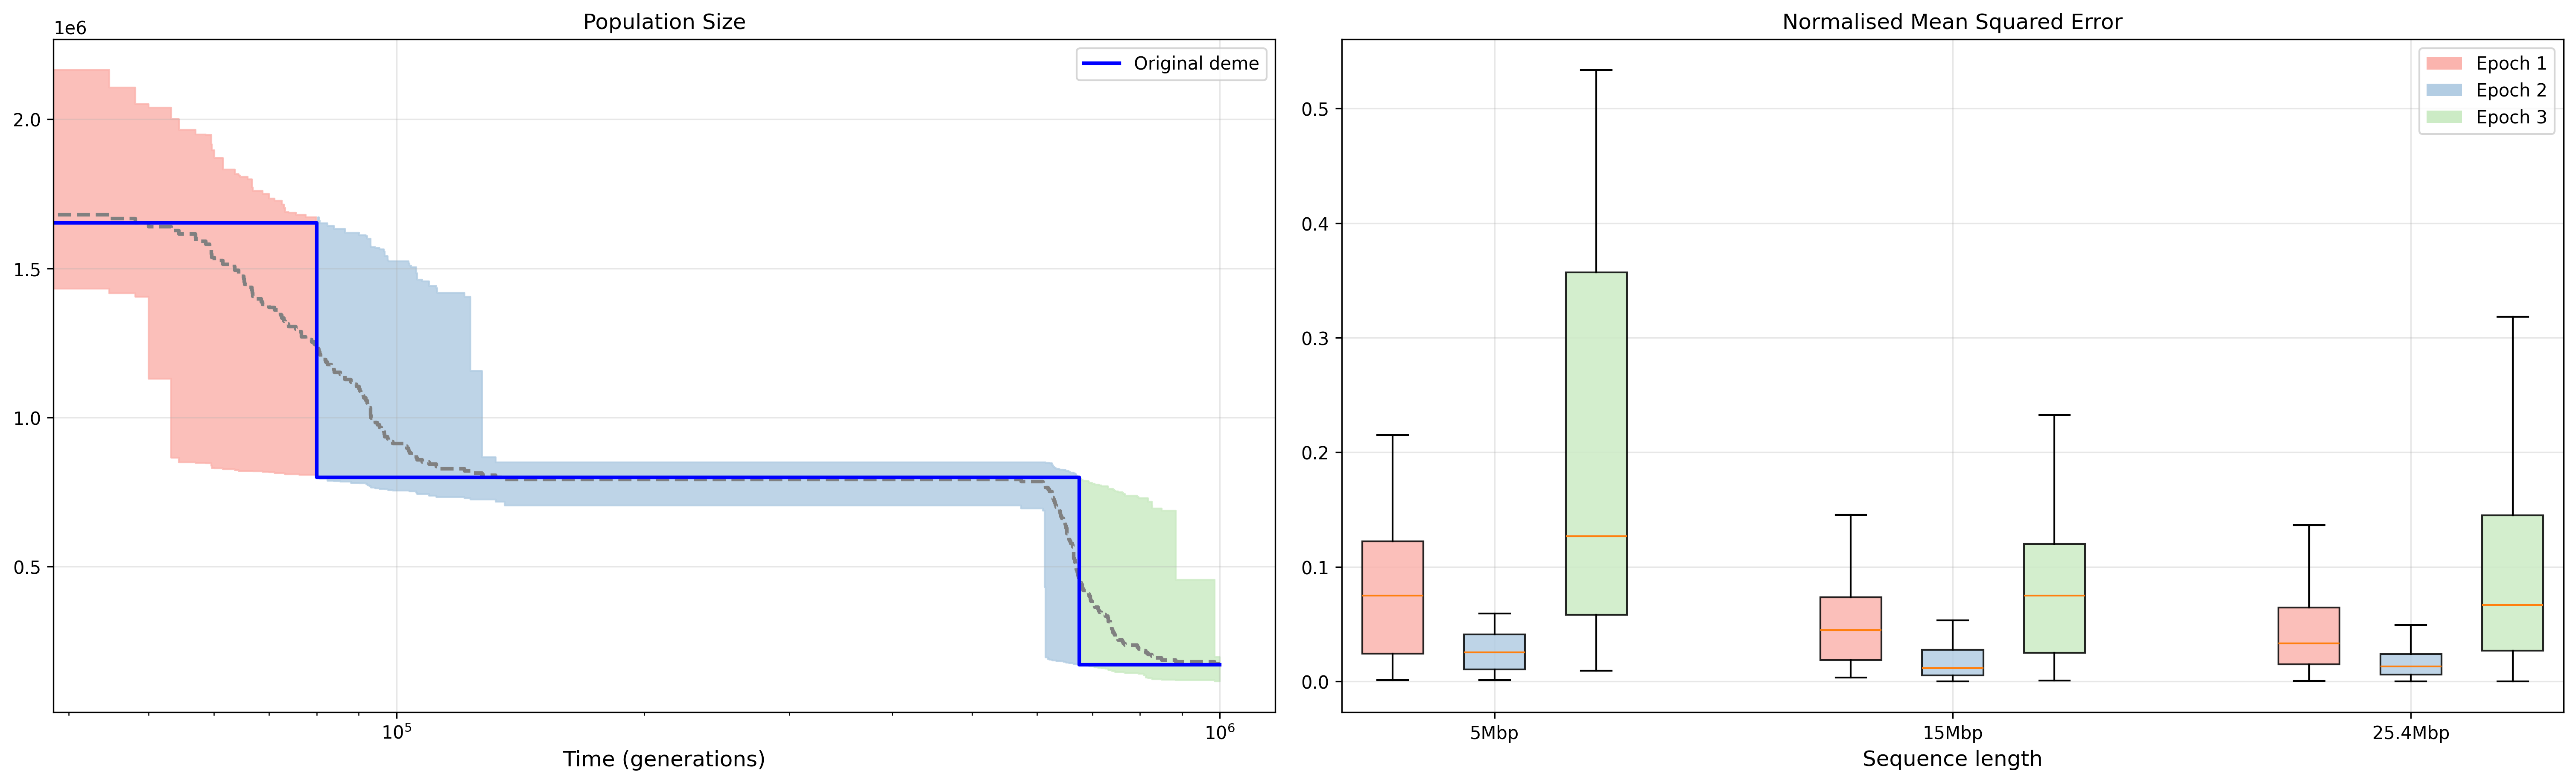
\includegraphics[width=\linewidth]{figures/combined_demes_combinedplot.png}

\caption{\textbf{The SMC(k) enables the use of whole chromosome simulations to
estimate of the uncertainty of point estimates of demographic histories}.
\textbf{(left) The demography history of the South African \textit{D.\
melanogaster} population}. The blue line represents the demography history
inferred by \citep{chen_sub-saharan_2024}. The dotted shows the average history
of $N_e$ change inferred across 100 simulated SMC(1) bootstrap replicates; the
associated 95\% confidence interval is shown as a gray sleeve. \textbf{(right)
The Root Mean Squared Error (RMSE) of epoch wise $N_e$ estimates decreases with
sequence length.} The distribution of RMSE for each simulated epoch for three
simulated sequence lengths.}

\label{fig:bootstrap}
\end{figure*}

\section{Methods}
% descibe version used etc to make Fig 3
All simulations were performed using \textit{msprime v1.4} on a 12th Gen Intel®
Core™ i5-1250P processor. ARG operations were supported by \textit{tskit v1.0}
\citep{jeffery_population-scale_2026}.

\subsection{Benchmarking} We averaged the execution time across 25 replicate
simulations, each consisting of two diploid samples of sequence length 25.28
Mbp and a recombination rate $r_{bp}= 1.045e-8$. This corresponds to direct
estimates of the map length of \textit{Drosophila} chromosome 2R \citep[][Table
2]{comeron2012}. We assumed a quadratic fit of the CwR execution time to
estimate the predicted execution time for \textit{Drosophila}.

\subsection{Comparing SMC(k) and the CwR} We simulated 100kbp of chromosome 2R
in \textit{D.\ melanogaster} ($r_{bp}=1.045e-8$). To measure the distribution
of ancestral material, for each of the following parameters, we simulated 10
ARG replicates of two diploid samples with a sequence length of 100kbp and a
population size of 1M  diploid individuals, four models: full CwR, SMC(500kb),
SMC' [SMC(1)], and the standard SMC model [SMC(0)]. To retain unary nodes, we
set the coalescing\_segments\_only flag in \textit{msprime} to \textit{false}.
Since \textit{msprime} stops simulating a local tree once a most recent common
ancestor (MRCA) is reached, unary nodes may be absent from some local trees if
they belong to a branch above the local MRCA. Therefore, we set the
stop\_at\_local\_mrca flag to false, ensuring that simulations continue until a
local MRCA is reached for all local trees. (Fig.  \ref{fig:stacked_bar}).

We measured similarity as \textit{tscompare v0.2}'s matched sequence span. For
different $k$ values (0 [SMC], 1 [SMC'], 1kbp, and 10kbp), we simulated 1,000
independent pairs of ARG, each consisting of one ARG simulated under the SMC(k)
model and one ARG simulated under the CwR model. Each ARG is made of two
diploid samples (Fig. \ref{fig:ts_inverse_matched_span}).

\subsection{Bootstrapping demographic inference} We simulated replicate
datasets under this inferred history under the SMC(1), each consisting of 20
haploid sequences of chromosome 2R (the sequence length was set to 25.28 bp)
and assumed a recombination rate of $r_\mathrm{bp} = 1.045e-08$. We used the
\texttt{tskit} \texttt{allele\_frequency\_spectrum} function to calculate the
mutation based unfolded SFS \citep{Ralph2020Stats}.
\textcolor{red}{FIXME: there's no (a) and (b) in the Figure, and anyway, isn't
this detail for the caption?}
Fig. \ref{fig:bootstrap}
(a) shows the simulated demography and the mean estimated demography from
SMC(1) simulated SFSs using blockbuster. Fig \ref{fig:bootstrap} (b) shows the
decrease in normalised mean squared error for the three demography epochs with
the increase of simulated sequence length.
\textcolor{red}{FIXME: this isn't methods? Do we need this methods section for
bootstrapping at all? It would make the Results section more concrete and would
allow to to mention the simulation times if we just inlined it}
 Using larger $k$ values, however,
does not affect inference accuracy significantly (supplementary
Fig.~\ref{fig:varyingK}).

\section{Discussion}

The SMC has usually been evaluated by asking how closely it reproduces
particular summaries of the CwR. For example, the close agreement between
SMC$^\prime$ and the CwR in pairwise coalescence times has established that the
approximation is highly accurate for many two-locus quantities
\citep{wilton_smc_2015}. Our results show that this agreement does not extend
uniformly to the structure of the ARG as a whole. Low-$k$ approximations
systematically reduce the genomic persistence of ancestral lineages, while
increasing $k$ progressively restores the long-range ancestral structure
generated by the CwR. This distinction has become visible because recent
developments in ARG representation and comparison allow properties of ancestry
to be studied directly rather than through low-dimensional summaries
\citep{wong_general_2024,fritze2026forest}. More generally, these results
suggest that there is no single useful definition of the accuracy of an SMC
approximation. An approximation may reproduce marginal genealogies and
two-locus statistics extremely well while differing substantially in other
properties of the same ARG. The SMC($k$) provides a convenient way to explore
this distinction because $k$ defines a controlled sequence of models between
the SMC and the CwR.

The practical importance of these differences must therefore depend on the
analysis being performed. Our \emph{Drosophila melanogaster} example
illustrates this point. Despite clear differences between SMC$^\prime$ and CwR
ARGs in their long-range ancestral structure, increasing $k$ has only a modest
effect on the uncertainty of the SFS-based demographic estimates considered
here. Thus, reproducing the full long-range structure of the CwR appears
unnecessary for this particular inferential task, and the computational gains
of SMC$^\prime$ make chromosome-scale parametric bootstrapping practical in a
parameter regime where doing so under the CwR is prohibitively expensive.
Other analyses may depend much more strongly on the structures that low-$k$
approximations remove. Methods based on long haplotypes, rare variants, or
properties of reconstructed ARGs, for example, may be sensitive to ancestral
relationships spanning much larger genomic distances.
The SMC($k$) allows us to move from asking
whether the SMC is ``accurate'' or not, to asking which properties of ancestry need to
be represented in high fidelity for the biological or inferential problem at hand.

\section{Data availability}

\section{Acknowledgments}
We thank Guillaume Achaz for helpful discussions.

\section{Funding}
HL, GB, DS, KL and JK are funded by EPSRC grant EP/X022595/1.

%\section{Conflicts of interest}
%Please either state that you have no conflicts of interest, or list relevant information here.  This would cover any situations that might raise any questions of bias in your work and in your article’s conclusions, implications, or opinions. Please see \url{https://academic.oup.com/journals/pages/authors/authors_faqs/conflicts_of_interest}.

\bibliography{paper}

\beginsupplement
\clearpage
\section*{Supplementary Information}

\begin{figure}[!h]
\centering
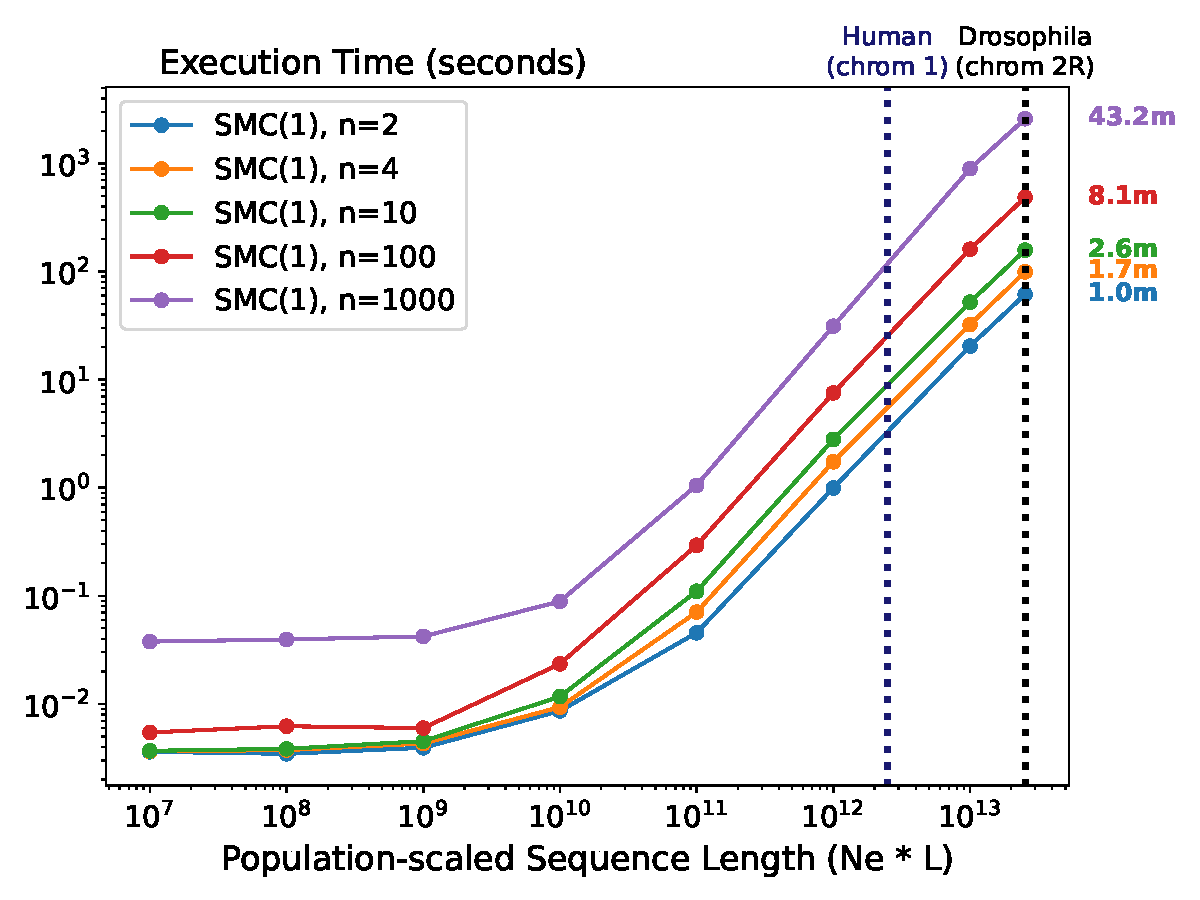
\includegraphics[width=\linewidth]{figures/speed_per_sample_size.pdf}
\caption{\textbf{Execution time scales with the number of simulated samples.} Execution time in seconds for the SMC(1) model across different population-scaled sequence lengths. Different line colours represent different numbers of simulated samples.}
\label{fig:speed_per_sample_size}
\end{figure}


\begin{figure}[!h]
\centering
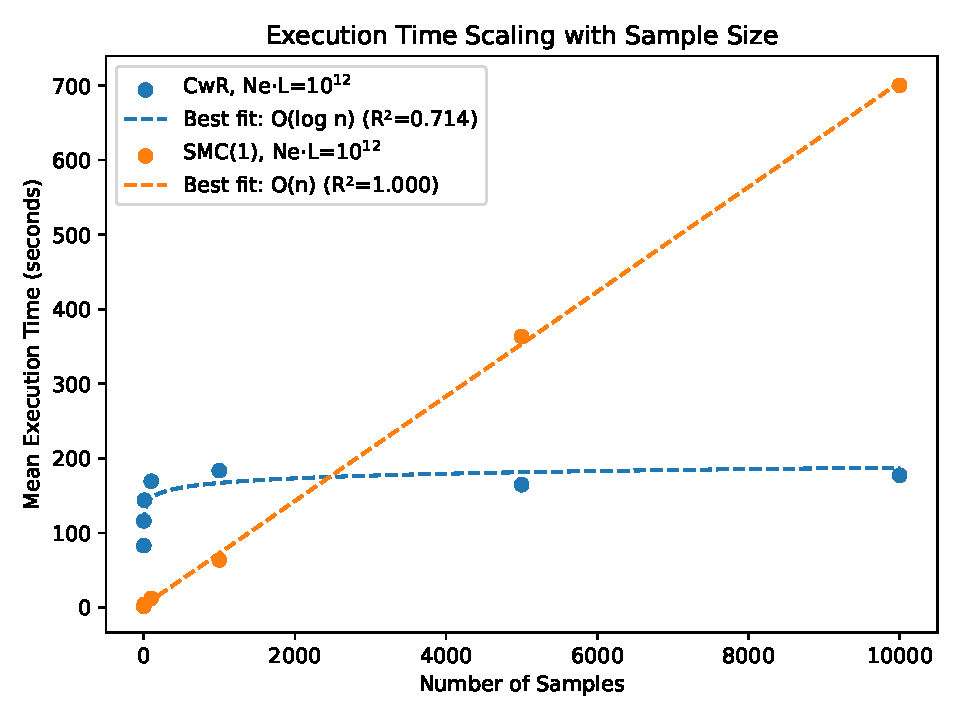
\includegraphics[width=\linewidth]{figures/scaling_with_sample_size_CwR_SMC(1)_nel1e+12.pdf}
\caption{\textbf{Excution time scales differently between the CwR model and the SMC(1) model.} Execution time scales linearly with sample size for the SMC(1) model ($O(n)$, orange), while it scales logarithmically with sample size for the CwR model ($O(logn)$, blue). }
\label{fig:scaling_sample_size}
\end{figure}


\begin{figure}[!h]
\centering
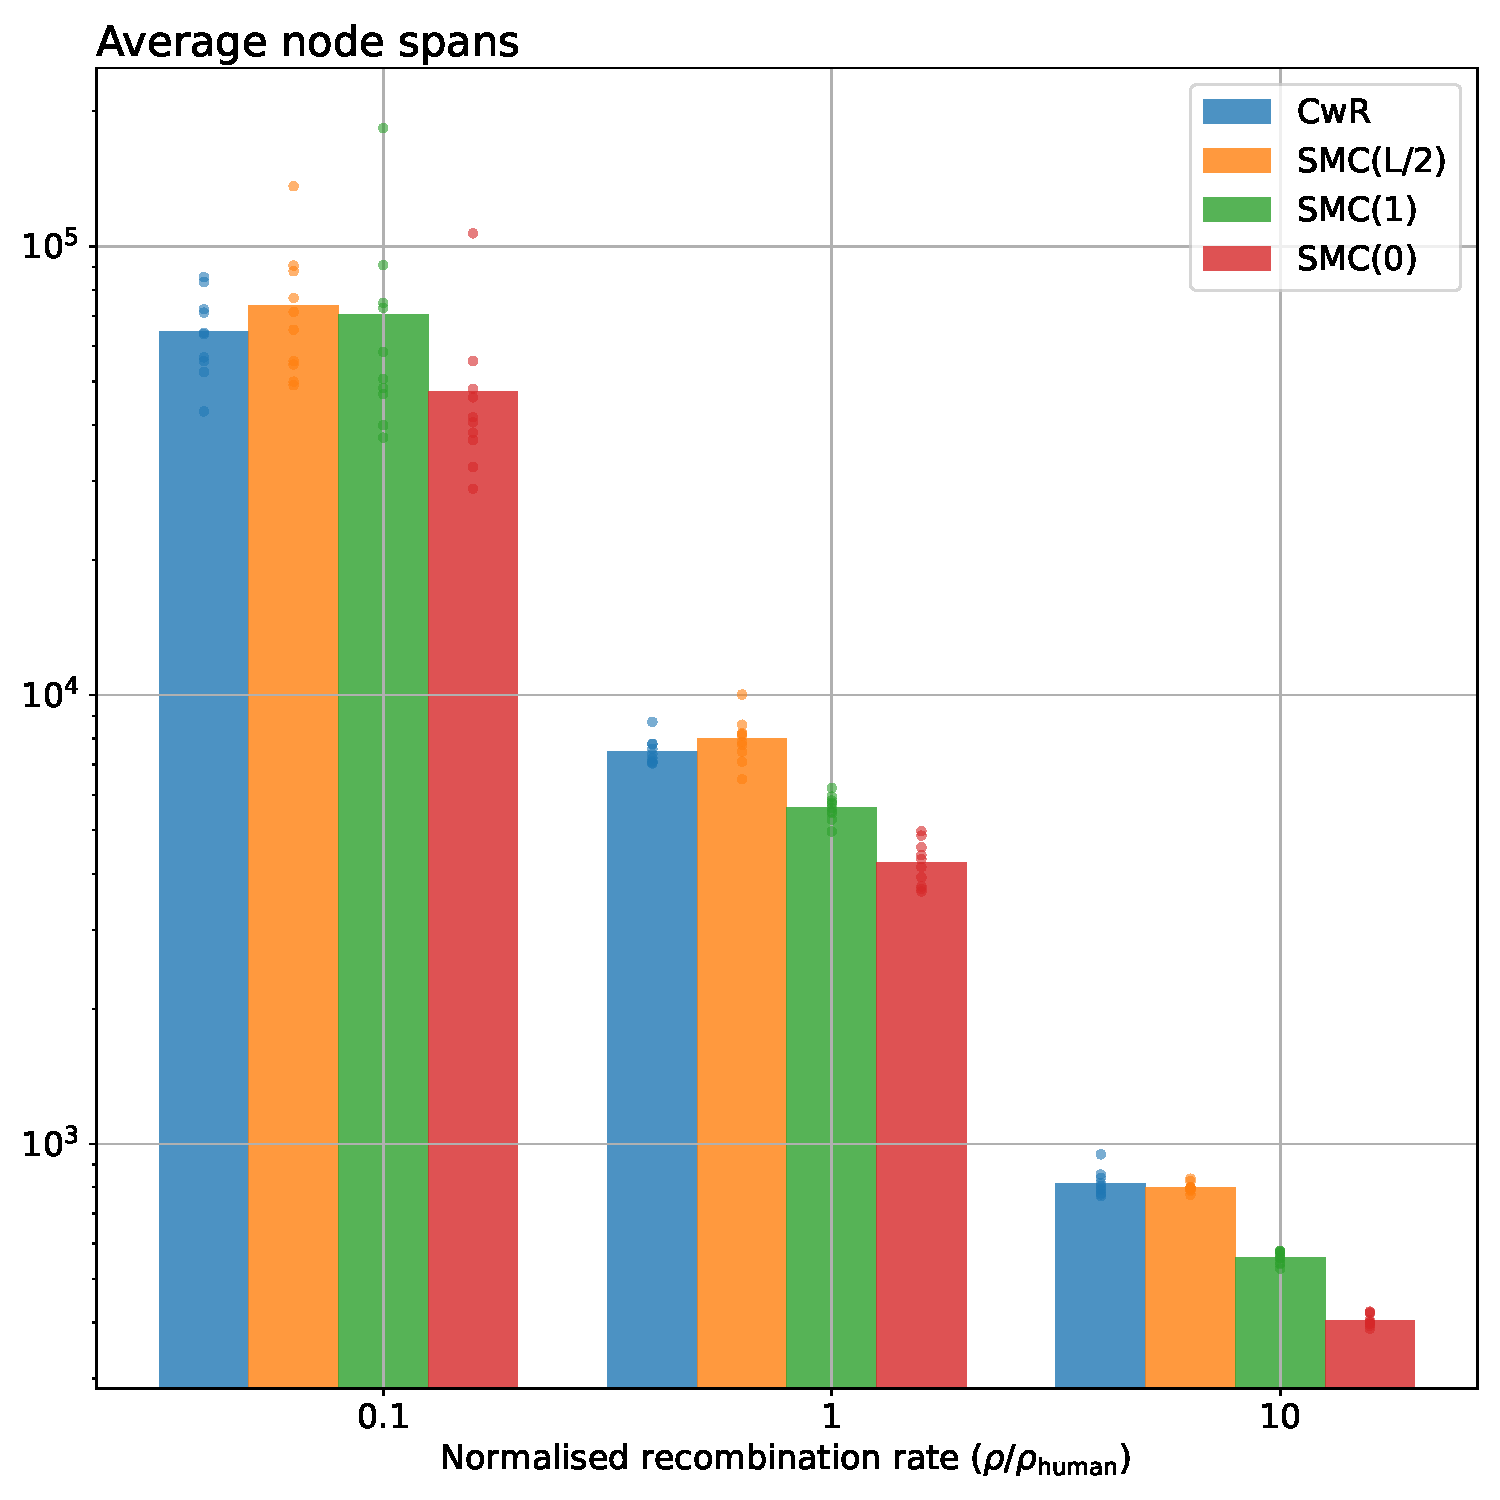
\includegraphics[width=\linewidth]{figures/single_paramaverage_hulls_2samples_segments_avg_l2_log.pdf}
\caption{\textbf{Average binary node spans are shorter for SMC(k) ARGs than for CwR ARGs.} The bar plot shows the average binary node span (n=10) for ARGs simulated under different models. The simulated sequence length is 1Mbp, population size is $10^6$ individuals, and recombination rate is $10^{-8}$ .}
\label{fig:avg_l2_log}
\end{figure}

\begin{figure}[!h]
\centering
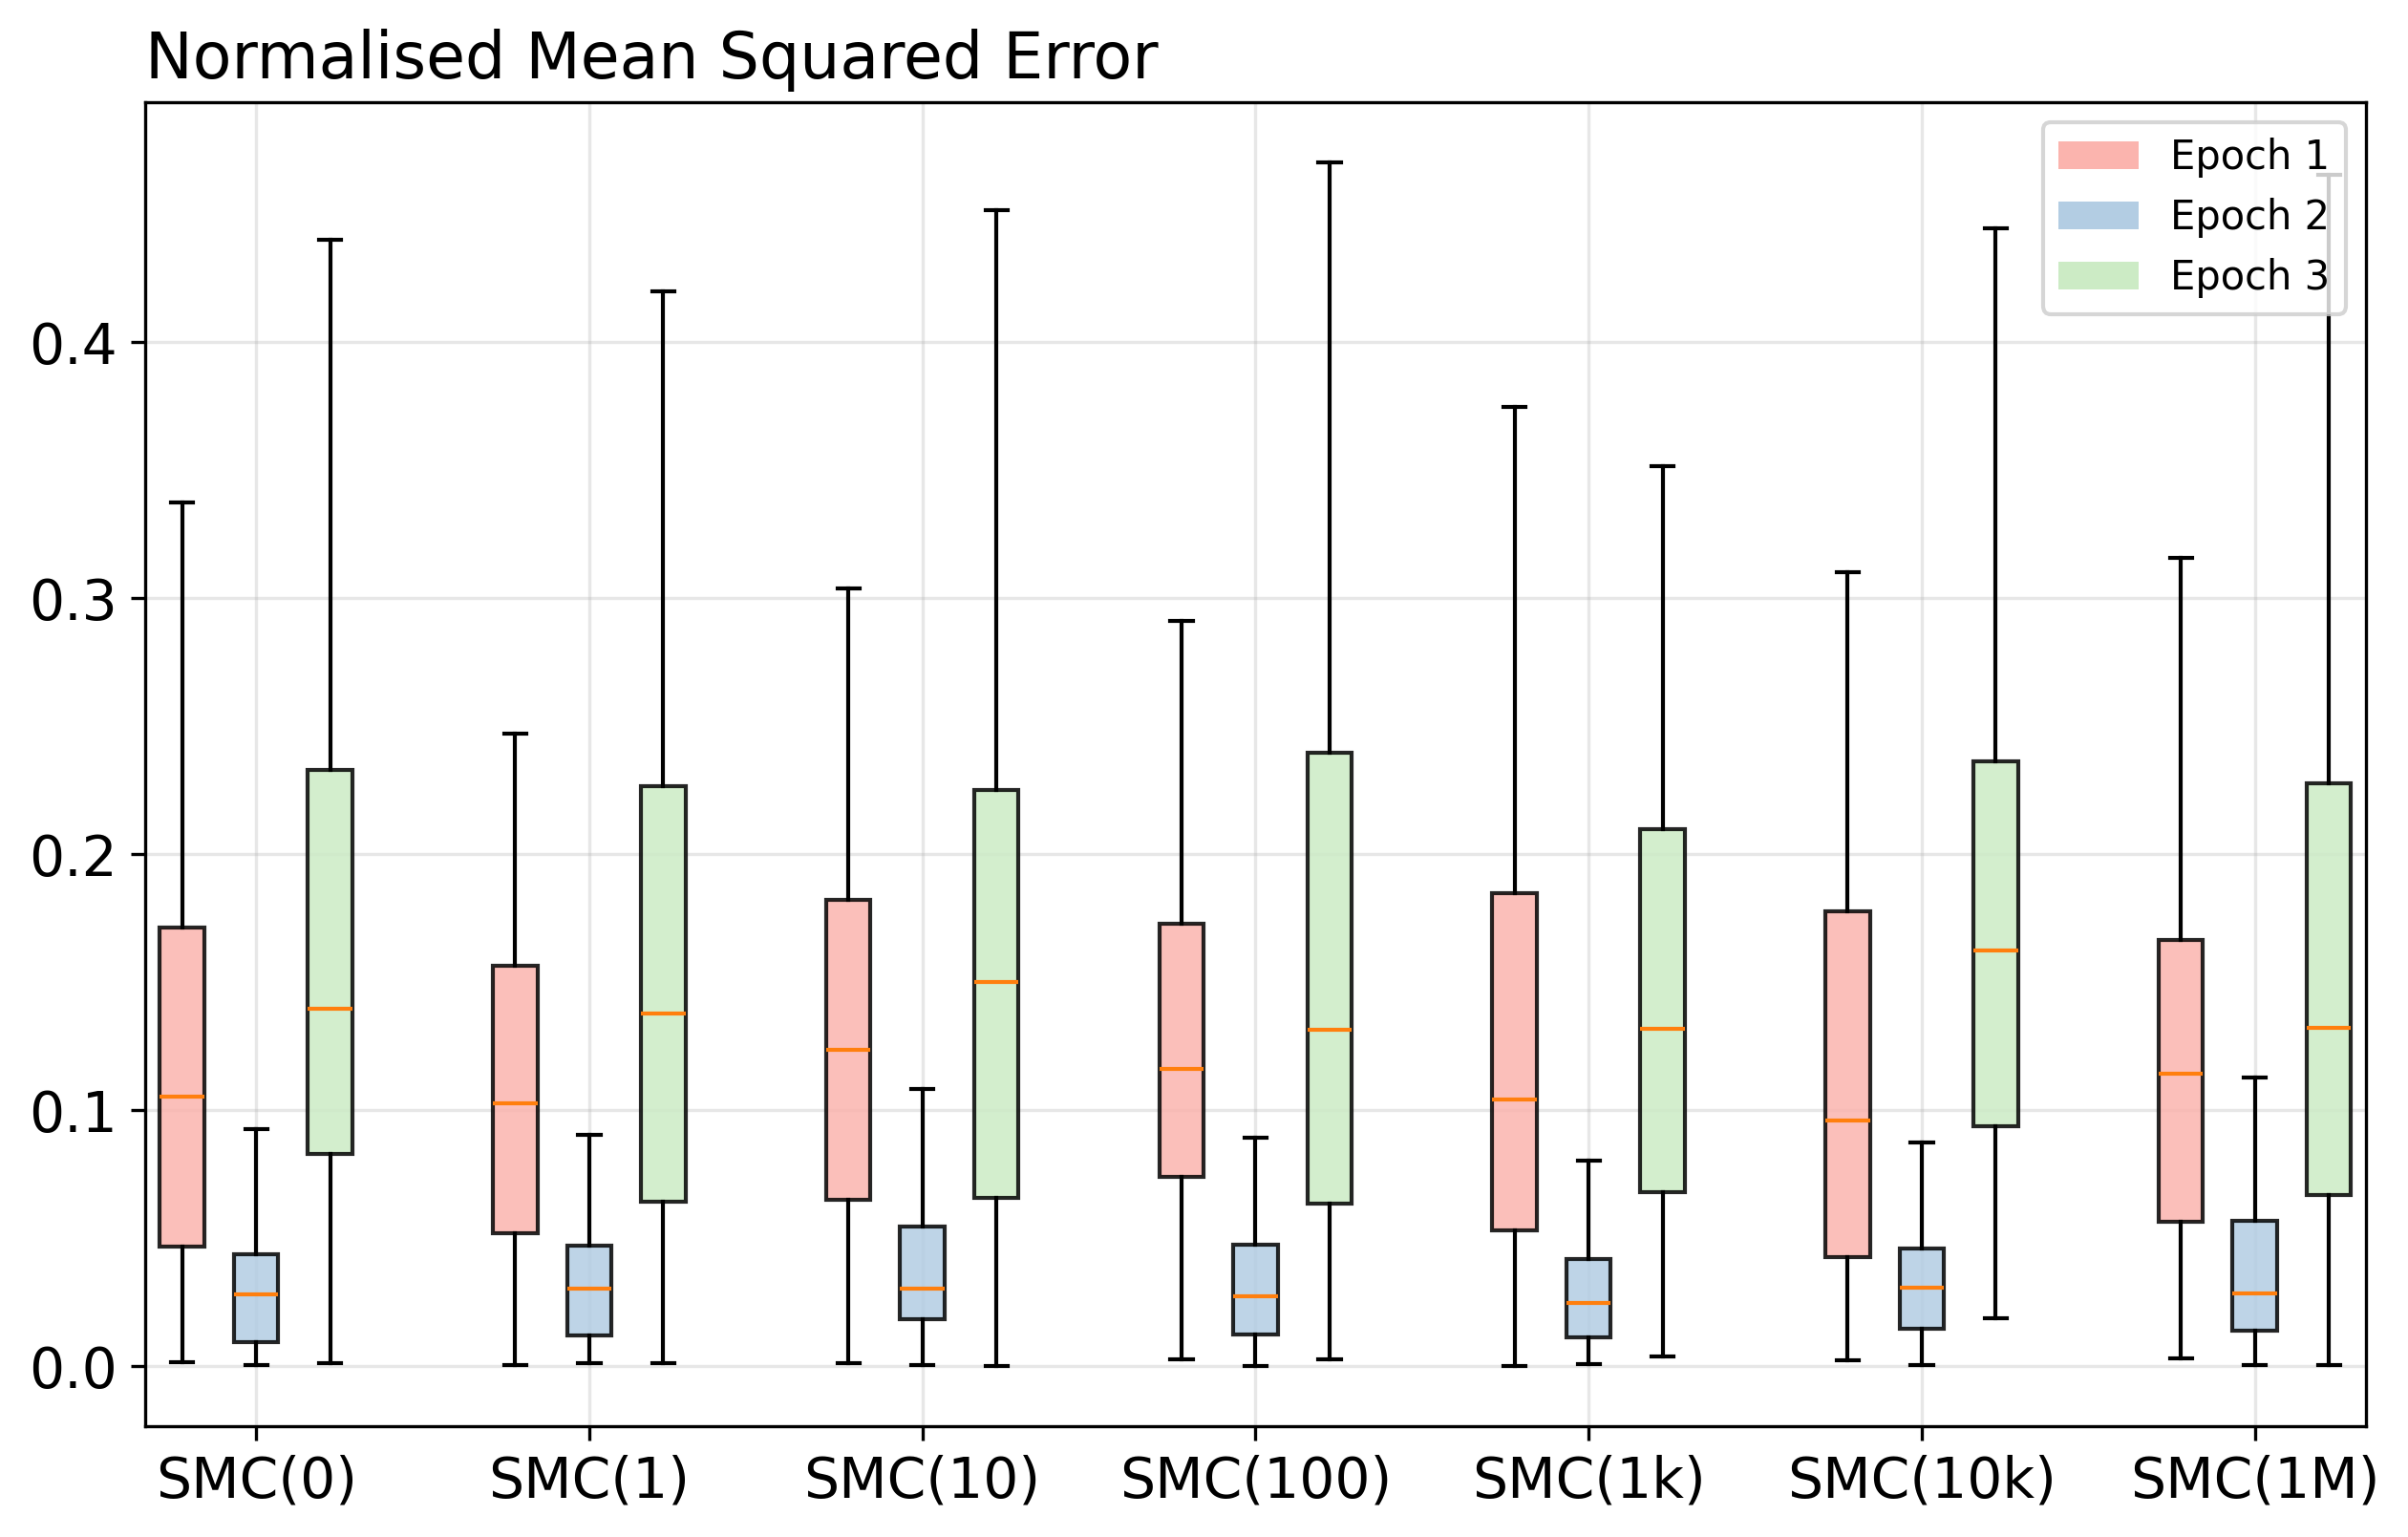
\includegraphics[width=\linewidth]{figures/combined_demes_SP_boxplots_only.png}
\caption{\textbf{Normalised Mean Squared Error in inferred population size is k value insensitive.} \textit{Blockbuster} population size inference from SFSs simulated under different SMC models. Increasing k value does not affect the quality of the population size inference.}
\label{fig:varyingK}
\end{figure}

\begin{figure}[!h]
\centering
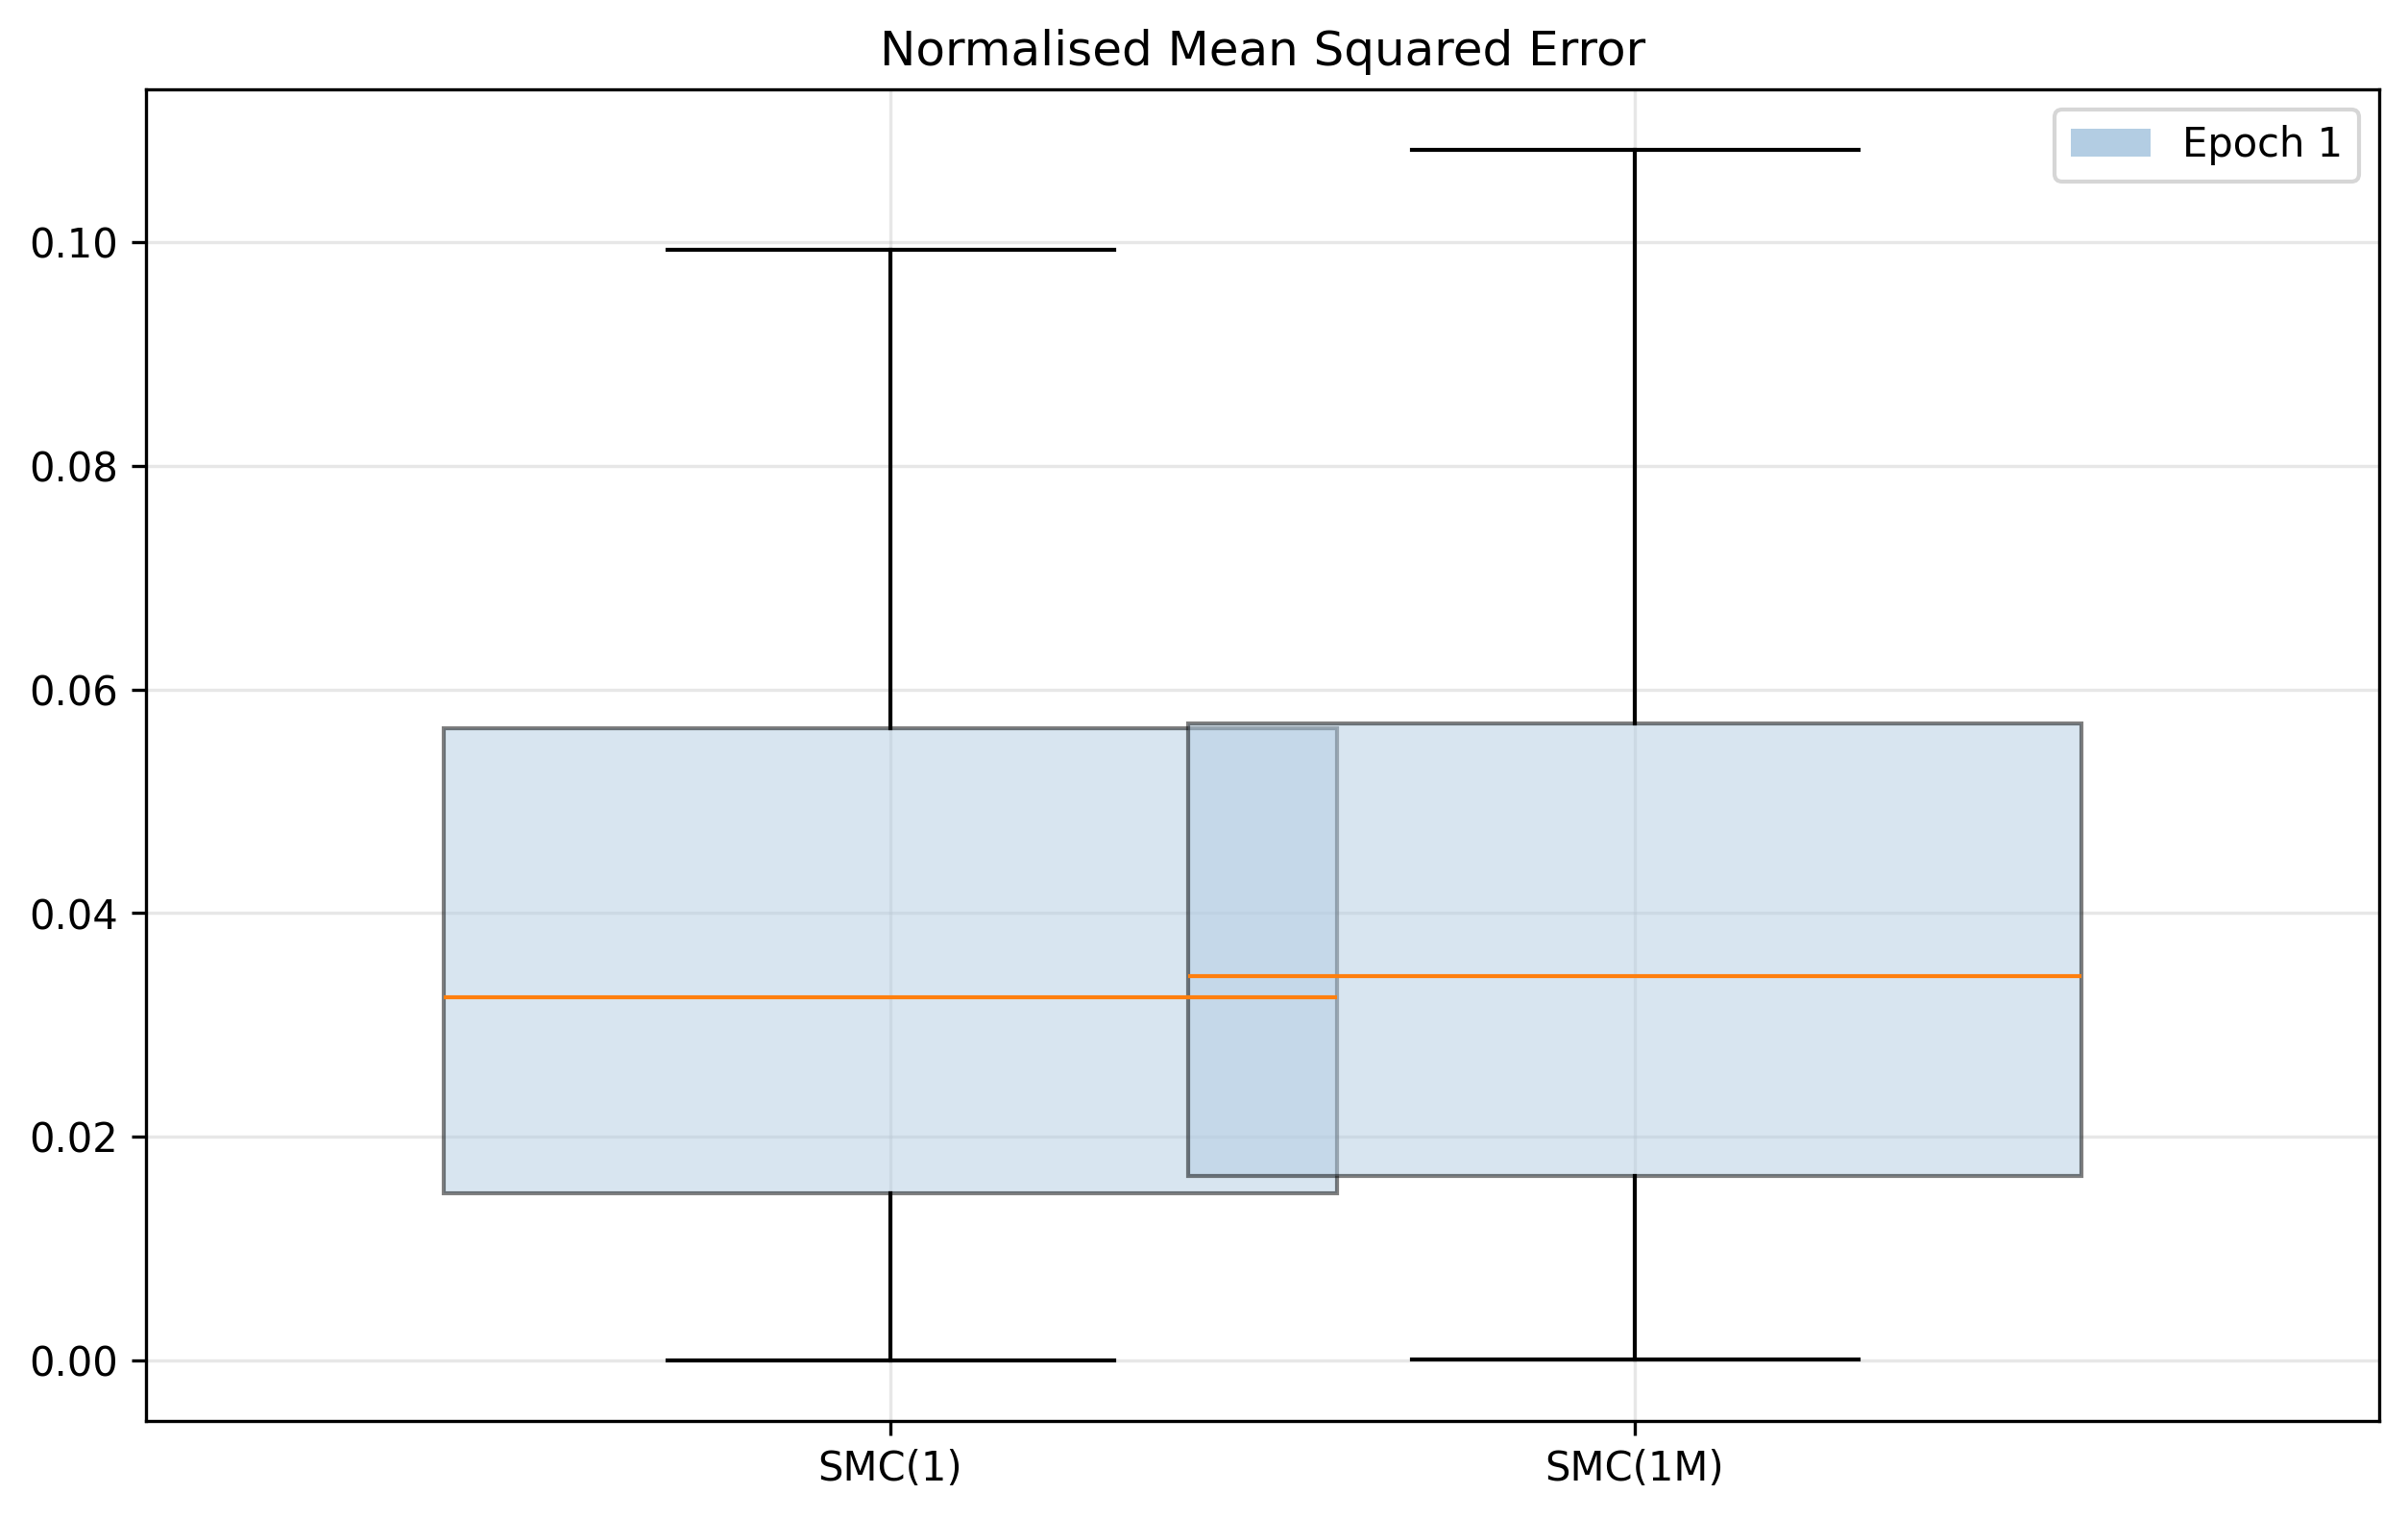
\includegraphics[width=\linewidth]{figures/combined_demes_compare_boxes.png}
\caption{\textbf{The variance in the Normalised Mean Squared error scales very modestly with k.} The variance of the Normalised Mean Squared Error of the inferred population size of a drosophila population simulated under the SMC(1) model and the SMC(1M) model.}
\label{fig:variance}
\end{figure}

\begin{figure}[!h]
\centering
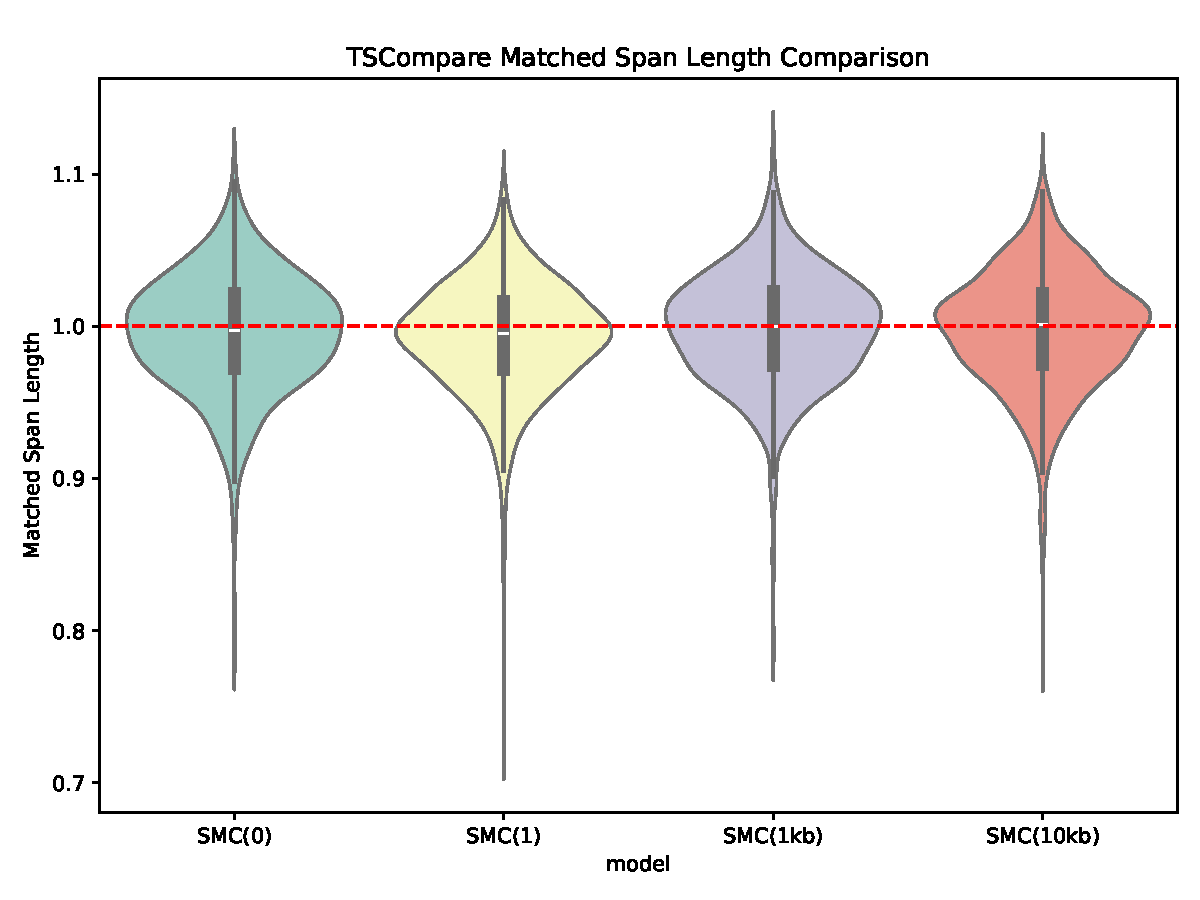
\includegraphics[width=\linewidth]{figures/tscompare_matched_span_length_comparison.pdf}
\caption{\textbf{The matched sequence spans of the SMC(K) ARGs to the CwR args does not depend on $k$.} The distribution of normalised similarity between ARGs simulated under the SMC(K) and CwR for different values of k. Similarity is measured in terms of the matched span length computed by tscompare
normalised by the similarity expected between two random ARGs simulated under the CwR.}
\label{fig:ts_matched_span}
\end{figure}


\begin{figure}[!h]
\centering
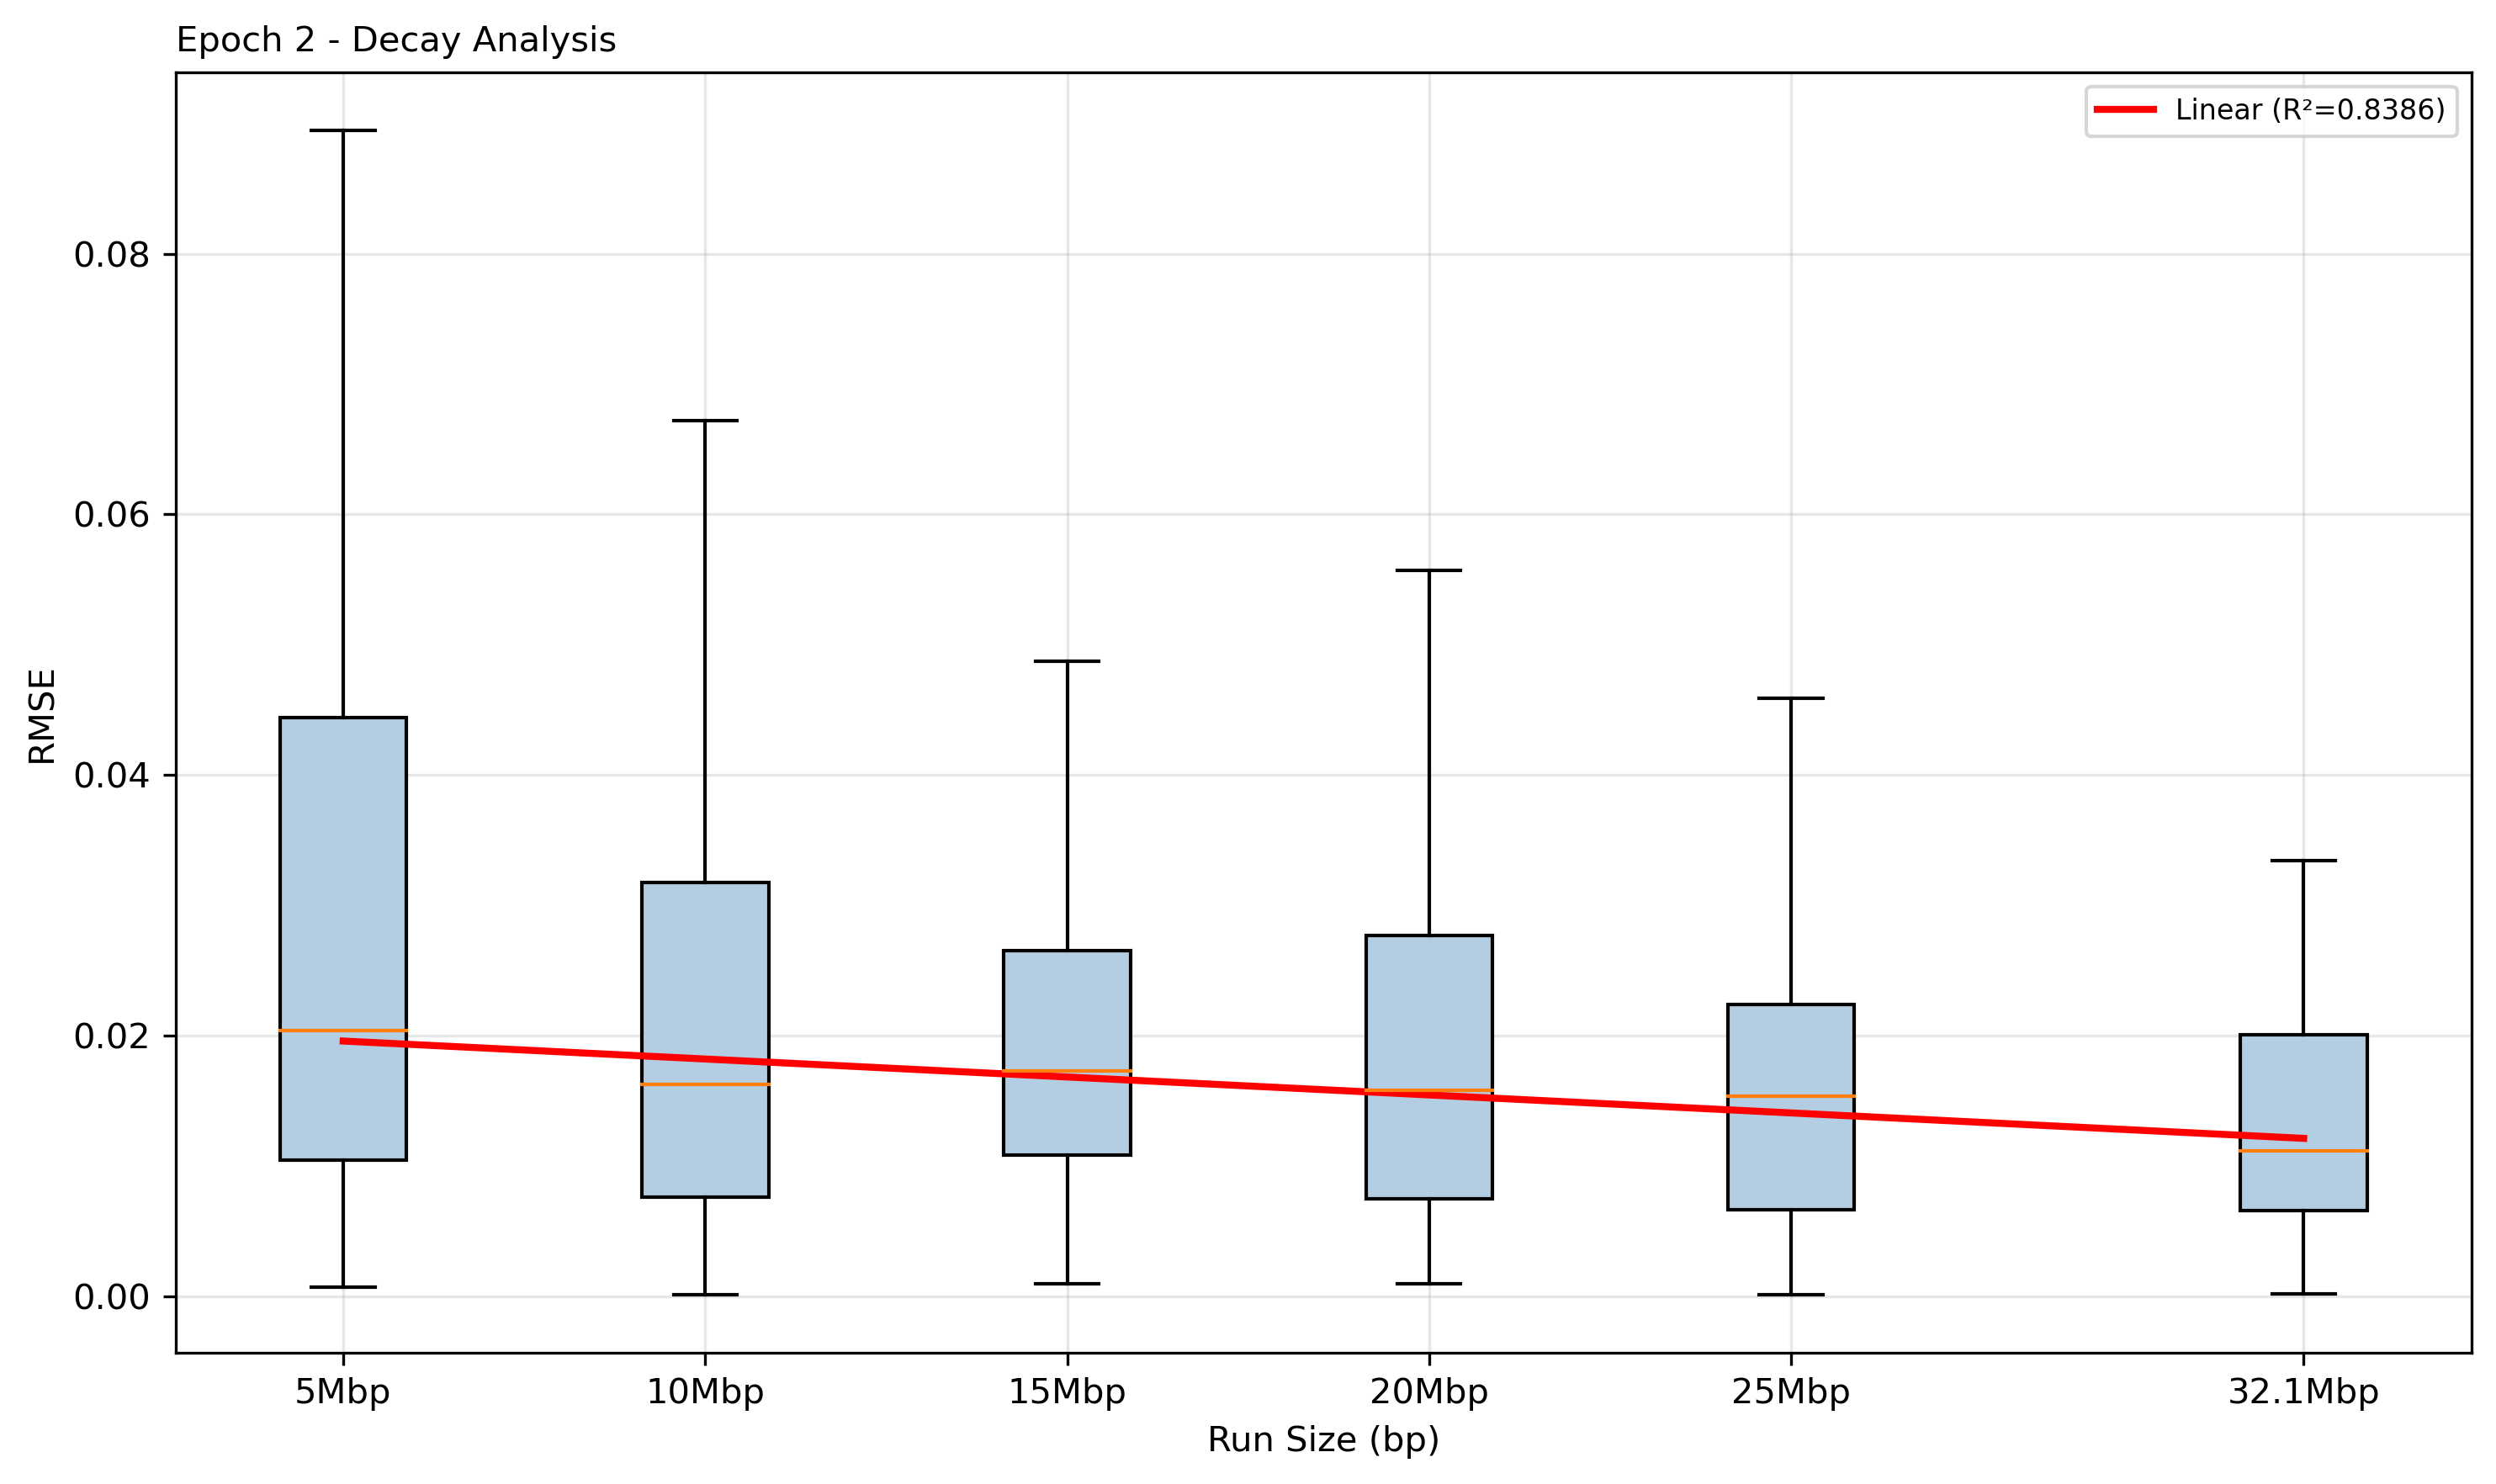
\includegraphics[width=\linewidth]{figures/error_decay_analysis.png}
\caption{RMSE error of inferred demography decreases linearly with simulated sequence length.}
\label{fig:error_decay_analysis}
\end{figure}


\begin{table}[h!]
\centering
\begin{tabular*}{\linewidth}{
@{\extracolsep{\fill}}
c|
>{\centering\arraybackslash}m{2cm}
>{\centering\arraybackslash}m{2cm}
>{\centering\arraybackslash}m{2cm}
}
\toprule
Node & Unary Span & Binary Span & Trapped non-ancestral Material Span\\
\midrule
3 & 5 & 0 & 0 \\
4 & 4 & 0 & 0 \\
5 & 3 & 0 & 2 \\
6 & 3 & 2 & 0 \\
7 & 2 & 3 & 0 \\
8 & 0 & 5 & 0 \\
\bottomrule
\end{tabular*}
\caption{\textbf{Sequence span per node example.} The sequence span per node in Fig:\ref{fig:illustration2} categorised by the type of ancestral material. }
\label{tab:nodespans}
\end{table}


\end{document}
